\documentclass[11pt]{article}

\usepackage[english]{babel}
\usepackage{indentfirst}
\usepackage{graphicx}
\usepackage{subfig}
\usepackage[section]{placeins}

\usepackage{xcolor}
\usepackage{listings}
\usepackage{float}
\usepackage{capt-of}

\definecolor{mGreen}{rgb}{0,0.6,0}
\definecolor{mGray}{rgb}{0.5,0.5,0.5}
\definecolor{mPurple}{rgb}{0.58,0,0.82}
\definecolor{backgroundColour}{rgb}{0.95,0.95,0.92}

\lstdefinestyle{CStyle}{
    backgroundcolor=\color{backgroundColour},   
    commentstyle=\color{mGreen},
    keywordstyle=\color{magenta},
    numberstyle=\tiny\color{mGray},
    stringstyle=\color{mPurple},
    basicstyle=\footnotesize,
    breakatwhitespace=false,         
    breaklines=true,                 
    captionpos=b,                    
    keepspaces=true,                 
    numbers=left,                    
    numbersep=5pt,                  
    showspaces=false,                
    showstringspaces=false,
    showtabs=false,                  
    tabsize=2,
    language=C
}






\begin{document}

\begin{titlepage}
	\begin{center}
		\vspace*{1cm}
		
		\Large
		\textbf{Protocolo de Ligação de Dados}
		
		\vspace{0.5cm}
		\large
		Primeiro Trabalho Laboratorial
		
		\vspace{1.5cm}
		
		\textbf{Hugo Miguel Monteiro Guimarães}\\
		\textbf{Pedro Varandas da Costa Azevedo da Ponte}
		
		\vspace{5cm}
		
		Trabalho realizado no âmbito da\\
		Unidade Curricular de Redes de Computadores
		
		\vspace{0.8cm}
		
		
\includegraphics[width=0.4 \textwidth]{feup_logo.png}
		
		\vspace{1.5cm}		
		
		\large
		Mestrado Integrado em Engenharia Informática e Computação\\
		Faculdade de Engenharia da Universidade do Porto\\
		Porto\\
		17 de novembro de 2020
	
	\end{center}
\end{titlepage}


\pagebreak
\tableofcontents

\pagebreak

\section*{Sumário}

Este trabalho foi realizado no contexto da cadeira Redes de Computadores, com o objetivo de implementar um protocolo de  ligação de dados através de uma porta série, permitindo a transmissão de um ficheiro entre 2 computadores.
 
Deste modo, o trabalho foi concluído com sucesso, dado que foi possível implementar uma aplicação que cumprisse os objetivos estabelecidos.


\section{Introdução}
Este trabalho pretende implementar um protocolo de ligação de dados baseado no guião fornecido, de modo a ser possível transferir ficheiros através de uma porta série.

O relatório pretende descrever detalhadamente a aplicação implementada, estando dividida nas seguintes secções:
\begin{description}
	\item[Arquitetura -] Descrição dos blocos funcionais e interfaces implementados.
	\item[Estrutura do Código -] Descrição das APIs, principais estruturas de dados, principais funções e a sua relação com a arquitetura.
	\item[Casos De Uso Principais -] Identificação dos principais casos de uso e da sequência de chamada de funções.
	\item[Protocolo De Ligação Lógica - ] Descrição dos principais aspetos funcionais do protocolo de ligação lógica e da sua estratégia de implementação com apresentação de extratos de código.
	\item[Protocolo De Aplicação - ] Descrição dos principais aspetos funcionais do protocolo de aplicação e da sua estratégia de implementação com apresentação de extratos de código.
	\item[Validação - ] Descrição dos testes efetuados com apresentação quantificada dos resultados.
	\item[Eficiência Do Protocolo De Ligação De Dados - ] Caracterização estatística da eficiência do protocolo de Stop\&Wait implementado.
	\item[Conclusões - ] Síntese da informação apresentada nas secções anteriores e reflexão sobre os objetivos de aprendizagem alcançados.
\end{description}

\section{Arquitetura}
O trabalho está divido em 2 secções fundamentais, o emissor e o recetor. Ambos incorporam a sua própria camada de ligação de dados e aplicação.

\section{Estrutura do Código}
O código está dividido em vários ficheiros.

Os ficheiros \textit{llfunctions.c} e \textit{stateMachines.c} são responsáveis pelo tratamento do protocolo da ligação de dados, sendo o  stateMachines.c unicamente responsável pela implementação das máquinas de estado de aceitação de mensagens.

O ficheiro \textit{application.c} é responsável pelo tratamento do protocolo de aplicação.

Os ficheiros \textit{emissor.c} e \textit{recetor.c} são responsáveis pelo fluxo de execução do programa, dos lados do emissor e recetor, respetivamente. Ambos contêm apenas a função main e todas as funções chamadas estão implementadas nos restantes ficheiros.


\textbf{emissor.c}
\begin{itemize}
	\item \textbf{main} - Controla os processos ao nível da camada da aplicação da parte do emissor e faz as chamadas às funções da camada de ligação.
\end{itemize}


\textbf{recetor.c}
\begin{itemize}
	\item \textbf{main} - Controla os processos ao nível da camada da aplicação da parte do recetor e faz as chamadas às funções da camada de ligação.
\end{itemize}


\textbf{llfunctions.c}
\begin{itemize}
	\item \textbf{llopen} - Do lado do emissor, envia uma trama de supervisão SET e recebe uma trama \textit{UA}, enquanto no lado do recetor este espera pela trama de controlo \textit{SET} enviada pelo emissor e responde com uma trama \textit{UA}.
	\item \textbf{llclose} -  Do lado do emissor, envia uma trama de supervisão \textit{DISC}, espera que o emissor responda com uma trama \textit{DISC} e envia uma trama \textit{UA}. No lado do recetor, este aguarda pela trama \textit{DISC} enviada pelo emissor, responde com uma trama \textit{DISC} e depois recebe uma trama \textit{UA}.
	\item \textbf{llwrite} - Faz o \textit{stuffing} das tramas I e envia-as, recebendo \textit{REJ} ou \textit{RR} como resposta.
	\item \textbf{llread} - Lê as tramas I enviadas pelo llwrite e envia uma resposta do tipo \textit{RR}, no caso das tramas I recebidas sem erros detetados no cabeçalho e no campo de dados, ou do tipo \textit{REJ}, no caso das tramas I sem erro detetado no cabeçalho, mas com erros no campo de dados.
	
\end{itemize}


\textbf{stateMachines.c}
\begin{itemize}
	\item \textbf{readSetMessage } -  Máquina de estados que recebe a trama \textit{SET} e verifica a sua correção.
	\item \textbf{readReceiverMessage } - Recebe as tramas \textit{REJ} e \textit{RR} enviadas pelo recetor e verifica a sua correção.
	\item \textbf{receiveUA} - Recebe as tramas \textit{UA} e verifica a sua correção.
	
	\item \textbf{receiverRead\_StateMachine} - Recebe as tramas I enviadas pelo emissor, verifica a sua correção, efetua o \textit{destuffing} necessário, guarda os dados contidos nas tramas I num novo array e envia uma trama \textit{REJ} ou \textit{RR} como resposta, dependendo da ocorrência de erros nas tramas recebidas ou no respetivo \textit{destuffing}.
	\item \textbf{receiveDISC } - Recebe as tramas \textit{DISC} e verifica a sua correção.
	
\end{itemize}

\textbf{application.c}
\begin{itemize}
	\item \textbf{parseControlPacket} -  Gera o pacote de controlo de um ficheiro para depois ser enviado.
	\item \textbf{parseDataPacket} - Codifica a mensagem num pacote de acordo com o protocolo estabelecido.
	\item \textbf{splitPacket} - Obtém uma porção da mensagem, de modo a enviar os dados sob a forma de uma trama I.
	\item \textbf{checkStart\_StateMachine} - Verifica se o primeiro pacote recebido pelo recetor é de facto o pacote de controlo de início.
	\item \textbf{checkEND} - Verifica se o pacote de controlo inicial é igual ao final.
	\item \textbf{assembleDataPacket} - Obtém os dados enviados pelo emissor através do pacote recebido pela porta série.

\end{itemize}

\textit{Para mais informações, consultar os anexos no final do relatório (Anexos I a XI).}


\section{Casos De Uso Principais}

Este trabalho laboratorial tem 2 casos de uso distintos: a interface e a transmissão do ficheiro.
A interface permite ao utilizador iniciar a aplicação. No lado do emissor, seleciona a porta de série que pretende utilizar (ex: \textbf{/dev/ttyS0}) e o ficheiro que pretende enviar (ex: \textbf{pinguim.png}). Do lado do recetor, basta apenas selecionar a porta de série a ser utilizada.

A transmissão do ficheiro, através da porta de série, entre os dois dispositivos, permite o estabelecimento da ligação entre os dispositivos, sendo o emissor responsável pela escolha do ficheiro a enviar. o emissor envia, trama a trama, os dados, sendo recebidos de igual forma pelo recetor que, antes de terminar a ligação, origina um ficheiro igual ao recebido originalmente.

\begin{itemize}
	\item Configuração da ligação e escolha do ficheiro a ser enviado pelo emissor;
	\item Estabelecimento da ligação entre o emissor e o recetor;
	\item Envio, trama a trama, dos dados por parte do emissor;
	\item Receção dos dados enviados pelo recetor, que os guarda num ficheiro com o mesmo nome do original à medida que os vai recebendo;
	\item Terminação da ligação.

\end{itemize}


\section{Protocolo De Ligação Lógica}

O objetivo do protocolo de ligação lógica é estabelecer a ligação estável e fiável entre os 2 computadores, utilizando a porta de série. Para isso, implementamos, tal como é referido no enunciado, as funções llopen, llread, llwrite e llclose.

\textit{Consultar o anexo XII para mais informações sobre as principais funções utilizadas para implementação do Protocolo de Ligação Lógica.}

\subsection{LLOPEN}

Esta função é responsável por estabelecer a ligação entre o emissor e o recetor através da porta de série.

Do lado do transmissor, esta função instala o alarme que vai ser utilizado ao longo da ligação, envia uma trama \textit{SET} ao recetor, ficando depois à espera que este envie na resposta uma trama do tipo \textit{UA}. Caso o recetor não responda passados 3 segundos, o emissor volta a reenviar a trama \textit{SET}, aguardando depois uma resposta do outro lado. Caso volte a ficar sem resposta ao fim dos 3 segundos, repete o envio mais uma vez e no caso de mais um insucesso o programa termina. Caso o recetor responda com a trama \textit{UA}, então a ligação é estabelecida.

Do lado do recetor, este aguarda o envio da trama \textit{SET} por parte do emissor e responde com o envio de uma trama do tipo \textit{UA}.

\textit{Consultar anexo V para mais informações sobre a implementação desta função.}

\subsection{LLWRITE}

A função llwrite é responsável pelo \textit{stuffing} e envio das tramas do tipo I.

Inicialmente, é acrescentado um cabeçalho à mensagem, de acordo com o protocolo descrito no guião. De seguida, é feito o \textit{stuffing} do \textit{BCC2} e da mensagem, pelo que a trama está pronta para ser enviada.

O processo de envio das tramas do tipo I está protegido por um alarme com 3 segundos de espera e 3 tentativas.

Após o envio, é esperada uma resposta pela parte do recetor, através do comando \textit{RR}, que simboliza que a trama foi transmitida corretamente, ou do comando \textit{REJ}, que indica problemas no envio da trama, originando um reenvio da trama original.

\textit{Consultar anexo V para mais informações sobre a implementação desta função.}

\subsection{LLREAD}

A função llread recebe as tramas do tipo I enviadas pelo emissor.

A trama recebida é lida e analisada através de uma máquina de estados, sendo feitas as verificações do cabeçalho e do campo de dados e realizado o respetivo \textit{destuffing} caso seja necessário.

Caso a trama recebida se trate de uma nova trama e não tenha erros no cabeçalho, mas possua erros no campo de dados, é enviada uma resposta do tipo \textit{REJ} para o emissor, pedindo uma retransmissão dessa trama. Caso contrário, é enviada uma resposta do tipo \textit{RR}.

Se a trama recebida não possuir erros no cabeçalho e no campo de dados, ou caso seja um duplicado, é confirmada ao emissor através de uma trama \textit{RR}.

Tramas com o cabeçalho errado são ignoradas, sem qualquer ação.

\textit{Consultar anexo V para mais informações sobre a implementação desta função.}



\subsection{LLCLOSE}

A função llclose tem como objetivo concluir a ligação entre o emissor e o recetor.

O emissor envia uma trama \textit{DISC}, esperando por uma resposta do emissor da mesma trama \textit{DISC}. Caso a receba, envia uma trama \textit{UA} para finalizar a ligação.

O emissor está protegido por um alarme de 3 tentativas de 3 segundos de espera, tal como as funções mencionadas anteriormente.

O recetor espera por uma trama \textit{DISC} e, caso a receba, envia de volta uma trama \textit{DISC}, esperando por uma trama \textit{UA} para finalizar a ligação.

\textit{Consultar anexo V para mais informações sobre a implementação desta função.}


\section{Protocolo De Aplicação}

O protocolo de aplicação permite a leitura de informação do ficheiro a enviar, fragmentando o ficheiro em tramas e preenchendo-o com um cabeçalho de controlo, sendo também capaz de descodificar a própria trama enviada.

\textit{Consultar o anexo XIII para mais informações sobre as principais funções utilizadas para implementação do Protocolo de Aplicação.}

Para que tal fosse implementado, recorremos às seguintes funções:

\begin{description}
	\item[OpenFile] Abre o ficheiro recebido e retorna os dados do ficheiro, assim como o seu tamanho.
	\item[ParseControlPacket] Gera um pacote de controlo do tipo \textit{START} ou \textit{END}, contendo o tamanho e o nome do ficheiro.
	\item[ParseDataPacket] Gera um pacote de dados, preenchendo-o com um cabeçalho contendo uma \textit{FLAG} de controlo, o número de pacotes, o tamanho do ficheiro e o respetivo fragmento do ficheiro a ser enviado.
	\item[SplitPacket] Divide o ficheiro em fragmentos mais pequenos.
	\item[CheckStart] Verifica se o pacote de controlo foi recebido corretamente e obtém deste o tamanho e o nome do ficheiro.
	\item[CheckEND] Compara o pacote de controlo do tipo \textit{START} enviado antes da transmissão dos dados com o do tipo \textit{END} recebido no final da transmissão, verificando se os campos com o tamanho e nome do ficheiro são iguais.
	\item[AssembleDataPacket] Retorna o campo de dados de um pacote.
	\item[CreateFile] Gera um ficheiro de acordo com os dados recebidos.
\end{description}


\section{Validação}

Foi testado o envio de vários ficheiros, incluindo ficheiros com uma elevada quantidade de dados, os quais foram enviados do emissor para o recetor corretamente, sem perda de informação.

Relativamente aos testes relacionados com a interrupção da ligação do cabo de série e geração de ruído, não fomos capazes de apresentar imagens relativas ao seu procedimento, porém, o seu sucesso foi comprovado na presença do docente no decurso da apresentação do projeto.

Para fortalecer ainda mais esta validação, recorremos ao envio de ficheiros simulando a ocorrência de erros no \textit{BCC} e no \textit{BCC2} com variação na percentagem de erros, à variação do tamanho dos pacotes , à variação das capacidades de ligação (\textit{baudrate}) e à geração de atraso de propagação simulado. Os resultados obtidos são a seguir apresentados.  


\section{Eficiência Do Protocolo De Ligação De Dados}

\subsection{Variação da capacidade de Baudrate}

Foi utilizada a imagem do pinguim (pinguim.png), com um tamanho de 35.4KB, sobre a qual se fez variar os valores do \textit{baudrate}.

Foi possível concluir que o aumento do \textit{baudrate} provoca uma diminuição da eficiência, embora o tempo de execução seja menor.

\textit{No anexo XIV encontram-se os dados por nós recolhidos e o respetivo gráfico que nos permitiram chegar a estas conclusões.}

\subsection{Variação do tamanho das tramas}

Utilizando uma imagem de tamanho 35.4KB e um \textit{baudrate} de 38400, fez-se variar o tamanho de envio das tramas em cada llwrite.

Foi possível concluir que o aumento do tamanho das tramas de envio provocou o aumento da eficiência, sendo o tempo de execução menor.

\textit{No anexo XV encontram-se os dados por nós recolhidos e o respetivo gráfico que nos permitiram chegar a estas conclusões.}

\subsection{Atraso no envio das tramas}

Utilizando uma imagem de tamanho 35.4KB, um \textit{baudrate} de 38400 e o envio de 128 bytes em cada trama, introduziu-se um atraso no envio de cada trama no llwrite, através da função \textit{usleep()}.

Tal como esperado, foi possível concluir que a introdução de um atraso no envio de tramas causa uma diminuição da eficiência do código, sendo o tempo de execução cada vez menor à medida que o atraso introduzido aumenta.

\textit{No anexo XVI encontram-se os dados por nós recolhidos e o respetivo gráfico que nos permitiram chegar a estas conclusões.}

\subsection{Geração de erros no cabeçalho e no campo de dados}

Foram criadas duas funções, generateRandomBCC e generateRandomBCC2, de modo a gerar erros no cabeçalho e campo de dados, respetivamente, a uma percentagem definida no ficheiro macros.h, através das macros BCC1ERRORRATE e BCC2ERRORRATE.

Utilizando uma imagem de tamanho 35.4KB, um \textit{baudrate} de 38400 e o envio de 128 bytes em cada trama, fez-se variar os valores de BCC1ERRORRATE e BCC2ERRORRATE.

Tal como esperado, foi possível concluir que o aumento da taxa de erros gerados no cabeçalho e campo de dados provocou uma diminuição da eficiência, também como um aumento do tempo de execução.

\textit{No anexo XVII encontram-se os dados por nós recolhidos e o respetivo gráfico que nos permitiram chegar a estas conclusões.}

\section{Conclusões}

Em suma, foi possível alcançar o objetivo proposto do trabalho, a implementação de um protocolo de ligação de dados fiável através de uma porta série, sendo possível enviar com sucesso ficheiros de diferentes tamanhos e extensões. O projeto encontra-se dividido em duas camadas distintas: camada de ligação e camada de aplicação, tal como fomos explicando ao longo deste relatório.

Através deste trabalho, foi possível compreender não só o processo de implementação de um protocolo de ligação de dados, mas também as condições que afetam a eficiência do protocolo, através da alteração do tamanho da trama de envio, do \textit{baudrate}, da quantidade de erros e do atraso no envio das tramas.

\newpage

\section{Anexos}

\subsection{Anexo I - emissor.h}
\begin{lstlisting}[style=CStyle]
#include <sys/types.h>
#include <sys/stat.h>
#include <fcntl.h>
#include <termios.h>
#include <stdio.h>

#include <errno.h>
#include <signal.h>
#include <stdlib.h>
#include <time.h>

#include <string.h>

#include "llfunctions.h"
#include "application.h"


/**
 * \brief main function that starts the proggram flow
 * @param argc argument count
 * @param argv char pointer array with the arguments
 */
int main(int argc, char** argv);

\end{lstlisting}

\pagebreak

\subsection{Anexo II - emissor.c}

\begin{lstlisting}[style=CStyle]
/*Non-Canonical Input Processing*/
#include "emissor.h"

extern unsigned int packetNumber;

int main(int argc, char** argv)
{
  int fd;

  if ((argc < 3) || ((strcmp("/dev/ttyS0", argv[1])!=0) && (strcmp("/dev/ttyS1", argv[1])!=0))) {
    printf("Usage:\tnserial SerialPort File path\n\tex: nserial /dev/ttyS1 \t filename.jpg \n");
    return -1;
  }

  /*
  Open serial port device for reading and writing and not as controlling tty
  because we don't want to get killed if linenoise sends CTRL-C.
  */
  
  struct timespec initialTime, finalTime;
  clock_gettime(CLOCK_REALTIME, &initialTime);

  if ((fd = open(argv[1], O_RDWR | O_NOCTTY )) < 0) {
    perror(argv[1]);
    return -2;
  }


  int fileNameSize = strlen(argv[2]);
  char* filename = (char*)malloc(fileNameSize);
  filename = (char*)argv[2];
  off_t fileSize = 0;
  int sizeControlPacket = 0;

  unsigned char *data = openFile(filename, &fileSize);

  // Dealing with the SET and UA
  if(llopen(fd, TRANSMITTER) == ERROR){
    puts("TRANSMITTER: Error on llopen");
    return -3;
  }

  // Start Control packet
  unsigned char *start = parseControlPacket(CT_START, fileSize, filename, fileNameSize, &sizeControlPacket);

  if(llwrite(fd, start, sizeControlPacket) != TRUE ){
    puts("TRANSMITTER: Error writing START control packet");
    return -4;
  }
  free(start);

  // Cicle to send packets
  int packetSize = PACKETSIZE;
  off_t index = 0;

  while(index < fileSize && packetSize == PACKETSIZE){
    unsigned char* packet = splitPacket(data, &index, &packetSize, fileSize);

    int length = packetSize;
    
    unsigned char* message =  parseDataPacket(packet, fileSize, &length);

    if(llwrite(fd, message, length) != TRUE){
      puts("TRANSMITTER: Error sending data packet");
      return -5;
    }

    printf("Sent packet number: %d\n", packetNumber);

    free(message);
  }


  // End Control packet
  unsigned char *end = parseControlPacket(CT_END, fileSize, filename, fileNameSize, &sizeControlPacket);

  if(llwrite(fd, end, sizeControlPacket) != TRUE ){
    puts("TRANSMITTER: Error writing END control packet");
    return -6;
  }
  free(end);


  if(llclose(fd, TRANSMITTER) == ERROR){
    puts("TRANSMITTER: Error on llclose");
    return -7;
  }

  clock_gettime(CLOCK_REALTIME, &finalTime);

  double accum = (finalTime.tv_sec - initialTime.tv_sec) + (finalTime.tv_nsec - initialTime.tv_nsec) / 1E9;

  printf("Seconds passed: %f\n", accum);

  sleep(1);
  close(fd);
  free(data);

  return 0;
}
\end{lstlisting}

\pagebreak

\subsection{Anexo III - recetor.h}

\begin{lstlisting}[style=CStyle]
/*Non-Canonical Input Processing*/

#include <sys/types.h>
#include <sys/stat.h>
#include <fcntl.h>
#include <termios.h>
#include <stdio.h>
#include <string.h>

#include <time.h>


// Created files

#include "llfunctions.h"
#include "application.h"
\end{lstlisting}

\pagebreak

\subsection{Anexo IV - recetor.c}

\begin{lstlisting}[style=CStyle]
#include "recetor.h"

extern unsigned int packetNumber;

int main(int argc, char** argv)
{
  int fd;
  off_t index = 0;

  if ( (argc < 2) || 
        ((strcmp("/dev/ttyS0", argv[1])!=0) && 
        (strcmp("/dev/ttyS1", argv[1])!=0) )) {
    printf("Usage:\tnserial SerialPort\n\tex: nserial /dev/ttyS1\n");
    return -1;
  }

/*
  Open serial port device for reading and writing and not as controlling tty
  because we don't want to get killed if linenoise sends CTRL-C.
*/

  struct timespec initialTime, finalTime;
  clock_gettime(CLOCK_REALTIME, &initialTime);
  
  fd = open(argv[1], O_RDWR | O_NOCTTY );
  if (fd <0) {
    perror(argv[1]); 
    return -2;
  }

  if(llopen(fd, RECEIVER) == ERROR){
    puts("Error on llopen");
    return -3;
  }

  unsigned char* start = malloc(0);
  unsigned int size, sizeStart;

  
  size = llread(fd,start);
  sizeStart = size;


  unsigned int fileSize = 0;
  unsigned int nameSize = 0;
  char *fileName  = (char *)malloc(0);

  if(checkStart(start,&fileSize,fileName,&nameSize) == ERROR){
    puts("Error on checkStart");
    return -4;
  }

  // Loop for reading all llwrites from the emissor
  unsigned char* dataPacket;
  unsigned int packetsRead = 0;
  unsigned int messageSize;

  unsigned char* final;

  unsigned char* result = (unsigned char*)malloc(fileSize); // Creates null pointer to allow realloc

  while(TRUE){
    unsigned int packetSize = 0;
    unsigned char* message = malloc(0);
    messageSize = 0;
    
    if((messageSize = llread(fd,message)) == ERROR){
      puts("Error on llread data packet ");
      return -5;
    }
    printf("message size = %d\n",messageSize);
    
    if(messageSize == 0){
      continue;
    } 
    else if (message[0] == CT_END){
      puts("Reached Control End Packet");
      final = (unsigned char*)malloc(messageSize);
      memcpy(final,message,messageSize);
      break;
    }
    
    packetsRead++;
    
    printf("Received packet number: %d\n", packetsRead);

    dataPacket = assembleDataPacket(message,messageSize,&packetSize);

    for(int i= 0; i < packetSize; i++){
      result[index + i] = dataPacket[i];
    }

    index += packetSize;

    free(dataPacket);
  }
  
  if(checkEND(start, sizeStart, final, messageSize) == 1) {
    puts("Start and End packets are different!");
    return -6;
  }

  printf("Received a file of size: %u\n", fileSize);

  // Creating the file to be rewritten after protocol
  createFile(result,fileSize,fileName);


  if(llclose(fd, RECEIVER) == ERROR){
    puts("Error on llclose");
    return -7;
  }


  clock_gettime(CLOCK_REALTIME, &finalTime);
  double accum = (finalTime.tv_sec - initialTime.tv_sec) + (finalTime.tv_nsec - initialTime.tv_nsec) / 1E9;
  printf("Seconds passed: %f\n", accum);
  sleep(1);

  free(fileName);
  free(result);

  close(fd);

  return 0;
}
\end{lstlisting}

\pagebreak

\subsection{Anexo V - llfunctions.h}

\begin{lstlisting}[style=CStyle]

#include <stdio.h>
#include <stdlib.h>
#include <unistd.h>
#include <sys/types.h>
#include <sys/stat.h>
#include <fcntl.h>
#include <termios.h>
#include <errno.h>
#include <signal.h>
#include <string.h>

#include "stateMachines.h"
#include "macros.h"

/**
 * \brief Deals with the protocol initiation establishment
 * @param fd file descriptor for the serial port to be used for the connection
 * @param status If 0, sends SET message and waits for UA, if 1, waits for set and sends UA
 * @return returns 0 upon sucess, -1 otherwise
 */
int llopen(int fd, int status);


/**
 * \brief gets BCC2
 * @param message gets BCC2 from this message
 * @param size message size
 * @return returns BCC2
 */
unsigned char getBCC2(unsigned char *mensagem, int size);

/**
 * \brief stuffs BCC2
 * @param bcc2 bcc2 char to be stuffed
 * @param size size of BCC2 after stuffing
 * @return returns the stuffed BCC2
 */
unsigned char* stuffBCC2(unsigned char bcc2,unsigned int *size);

/**
 * \brief Sends an I packet from a message from buffer to the serial port
 * @param fd fiel desriptor of the serial port
 * @param buffer containing the messsage to be sent
 * @param length length of the message to be sent
 * @return TRUE(1) upon sucess, FALSE(0) upon failure
 */
int llwrite(int fd, unsigned char *buffer, int length);

/**
 * \brief Reads an I packets sent trough the serial port
 * @param fd file descriptor for the serial port
 * @param buffer buffer read from the serial port
 * @return size of the read buffer
 */
unsigned int llread(int fd, unsigned char *buffer);

/**
 * \brief Termination of the protocol by serial port
 * @param fd file descriptor of the serial port
 * @param status if 0, acts as sender. if 1, acts as receiver for the termination protocl
 * @return returns 0 upon sucess, -1 otherwise
 */
int llclose(int fd, int status);

/**
 * \brief handles the alarm
 * @param signo signal number to be handled
 */
void alarmHandler(int signo);


unsigned char* generateRandomBCC(unsigned char* packet, int packetSize);

unsigned char* generateRandomBCC2(unsigned char* packet, int packetSize);

\end{lstlisting}

\pagebreak

\subsection{Anexo VI - llfunctions.c}

\begin{lstlisting}[style=CStyle]
#include "llfunctions.h"


struct termios oldtio,newtio;

volatile int STP=FALSE;
extern unsigned char rcv;
int counter = 0;
int trama = 0;
extern int res;


int llopen(int fd, int status) {
    
    if (tcgetattr(fd, &oldtio) == -1) { /* save current port settings */
        perror("llopen: tcgetattr");
        return ERROR;
    }

    bzero(&newtio, sizeof(newtio));
    newtio.c_cflag = BAUDRATE | CS8 | CLOCAL | CREAD;
    newtio.c_iflag = IGNPAR;
    newtio.c_oflag = 0;

    /* set input mode (non-canonical, no echo,...) */
    newtio.c_lflag = 0;

    newtio.c_cc[VTIME]    = 20;   /* inter-character timer unused */
    newtio.c_cc[VMIN]     = 0;   /* blocking read until 0 chars received */

    /* 
    VTIME e VMIN devem ser alterados de forma a proteger com um temporizador a 
    leitura do(s) proximo(s) caracter(es)
    */

    tcflush(fd, TCIOFLUSH);

    if (tcsetattr(fd,TCSANOW,&newtio) == -1) {
        perror("tcsetattr");
        return ERROR;
    }

    puts("New termios structure set");


    if(status == TRANSMITTER) {

        // Installing Alarm Handler
        if(signal(SIGALRM, alarmHandler) || siginterrupt(SIGALRM, 1)){
            puts("Signal instalation failed");
            return ERROR;
        }

        counter = 0;
        do{
            int wr;
            if((wr = sendMessage(fd, C_SET)) != ERROR){
                printf("llopen: C_SET message sent: %d \n", wr);
            }
            else{
                puts("llopen: Error sending message");
            }

            alarm(TIMEOUT); // Call an alarm to wait for the message

            if(receiveUA(fd) == TRUE){
                puts("TRANSMITTER: UA received\n");
                STP = TRUE;
                counter = 0;
                alarm(0);
            }

        }while(STP == FALSE && counter < MAXTRIES);
    }
    else if(status == RECEIVER) {
        if(readSetMessage(fd) == TRUE) {
            puts("RECEIVER: Read SET message correctly");
            if(sendMessage(fd, C_UA) == -1) {
                fprintf(stderr, "llopen - Error writing to serial port (Receiver)\n");
                return ERROR;
            }
            else {
                puts("RECEIVER: Sent UA message");
            }
        }
        else {
            fprintf(stderr, "llopen - Error reading from serial port (Receiver)\n");
            return ERROR;
        }
    }
    return 0;
}

unsigned char getBCC2(unsigned char *mensagem, int size){

    unsigned char bcc2 = mensagem[0];
    
    for(int i = 1; i < size; i++){
        bcc2 ^= mensagem[i];
    }
    return bcc2;
}

unsigned char* stuffBCC2(unsigned char bcc2, unsigned int *size){
    unsigned char* stuffed;
    if(bcc2 == FLAG){
        stuffed = malloc(2 * sizeof(unsigned char));
        stuffed[0] = ESCAPE_BYTE;
        stuffed[1] = ESCAPE_FLAG; 
        (*size) = 2;
    }
    else if(bcc2 == ESCAPE_BYTE){
        stuffed = malloc(2 * sizeof(unsigned char));
        stuffed[0] = ESCAPE_BYTE;
        stuffed[1] = ESCAPE_ESCAPE;
        (*size) = 2; 
    }
    else{
        stuffed = malloc(sizeof(unsigned char));
        stuffed[0] = bcc2;
        (*size) = 1;
    }
    
    return stuffed;
}

int llwrite(int fd, unsigned char *buffer, int length) {
    unsigned char bcc2;
    unsigned int sizebcc2 = 1;
    unsigned int messageSize = length+6;
    unsigned char *bcc2Stuffed = (unsigned char *)malloc(sizeof(unsigned char));
    unsigned char *message = (unsigned char *)malloc(messageSize * sizeof(unsigned char));

    bcc2 = getBCC2(buffer, length);
    bcc2Stuffed = stuffBCC2(bcc2, &sizebcc2);

    
    // Start to fill the message
    message[0] = FLAG;
    message[1] = A_EE;
    if(trama == 0){
        message[2] = NS0;
    }
    else{
        message[2] = NS1;
    }
    message[3] = message[1] ^ message[2];

    // Start to read from 4 and size depends on the message to send
    int i = 4;
    for(int j = 0; j < length; j++){
        if(buffer[j] == FLAG){
            message = (unsigned char *)realloc(message, ++messageSize);
            message[i] = ESCAPE_BYTE;
            message[i + 1] = ESCAPE_FLAG;
            i+=2;
        }
        else if(buffer[j] == ESCAPE_BYTE){
            message = (unsigned char *)realloc(message, ++messageSize);
            message[i] = ESCAPE_BYTE;
            message[i+1] = ESCAPE_ESCAPE;
            i+=2;
        }
        else{
            message[i] = buffer[j];
            i++;
        }
    }

    if(sizebcc2 == 2){
        message = (unsigned char *)realloc(message, ++messageSize);
        message[i] = bcc2Stuffed[0];
        message[i + 1]  = bcc2Stuffed[1];
        i+=2;
    }
    else{
        message[i] = bcc2;
        i++;
    }
    message[i] = FLAG;

    // Packet I filled
    // printMessage
    for(int j = 0; j < messageSize; j++){
        printf("message[%d] = 0x%X\n", j, message[j]);
    }
    

    counter = 0;
    STP = FALSE;

    // Send packet
    do {

        unsigned char* copyBcc = (unsigned char *)malloc(messageSize);
        unsigned char* copyBcc2 = (unsigned char *)malloc(messageSize);

        copyBcc = generateRandomBCC(message,messageSize);
        copyBcc2 = generateRandomBCC2(copyBcc,messageSize);


        int wr = write(fd, copyBcc2, messageSize);

        printf("TRANSMITTER: SET message sent: %d bytes sent\n", wr);

        alarm(TIMEOUT);

        readReceiverMessage(fd);
    
        // Handle rcv
        if((rcv == RR0 && trama == 1) || (rcv == RR1 && trama == 0)) {
            counter = 0;
            trama = (trama + 1) % 2;
            STP = FALSE;
            alarm(0);
            if(rcv == RR0) {
                puts("TRANSMITTER: Received RR0");
            }
            else {
                puts("TRANSMITTER: Received RR1");
            }
            break;
        }

        else if(rcv == REJ0 || rcv == REJ1) {
            STP = TRUE;
            if(rcv == REJ0) {
                puts("TRANSMITTER: Received REJ0");
            }
            else {
                puts("TRANSMITTER: Received REJ1");
            }
        }

        else if(res == 0) {
            puts("TRANSMITTER: Don't read any message from Receiver");
            STP = TRUE;
        }

        else {
            puts("TRANSMITTER: Received an invalid message");
        }

    } while(STP && counter < MAXTRIES); 

    if(counter >= MAXTRIES) {
        return FALSE;
    }
    else {
        return TRUE;
    }
}

unsigned int llread(int fd, unsigned char* buffer) {

    unsigned int size = 0;
    receiverRead_StateMachine(fd,buffer, &size);

    printf("size llread = %d\n",size);

    return size;
}

int llclose(int fd, int status) {
    if(status == TRANSMITTER) {

        counter = 0;
        STP = FALSE;
        
        do {
            int wr;
            if((wr = sendMessage(fd, C_DISC)) != ERROR){
                puts("TRANSMITTER: C_DISC message sent");
            }
            else{
                puts("TRANSMITTER: Error sending C_DISC message");
            }

            alarm(TIMEOUT); // Call an alarm to wait for the message

            if(receiveDISC(fd) == 0 && res != 0){
                puts("TRANSMITTER: C_DISC received");
                STP = TRUE;
                counter = 0;
                alarm(0);
            }
        } while(STP == FALSE && counter < MAXTRIES);

        if(sendMessage(fd, C_UA)) {
            puts("TRANSMITTER: Send UA");
        }
        tcsetattr(fd, TCSANOW, &oldtio);
    }

    else if(status == RECEIVER) {
        if (receiveDISC(fd) == 0) {
            puts("RECEIVER: Read DISC");
            if(sendMessage(fd, C_DISC)) {
                puts("RECEIVER: Send DISC");
                if(receiveUA(fd) == TRUE) {
                    puts("RECEIVER: Read UA");
                }
                
                else {
                    fprintf(stderr, "llclose- Error reading UA message (Receiver)\n");
                    return ERROR;
                }
            }

            else {
                fprintf(stderr, "llclose- Error writing DISC message to serial port (Receiver)\n");
                return ERROR;
            }
        }

        else {
            fprintf(stderr, "llclose - Error reading DISC message (Receiver)\n");
            return ERROR;
        }
        tcsetattr(fd, TCSANOW, &oldtio);
    }
    return 0;
}



void alarmHandler(int signo){

  counter++;
  if(counter >= MAXTRIES){
    printf("Exceeded maximum amount of tries: (%d)\n", MAXTRIES);
    exit(0);
  }
  return ;
}



unsigned char* generateRandomBCC(unsigned char* packet, int packetSize){
    unsigned char* copy = (unsigned char *)malloc(packetSize);
    memcpy(copy,packet,packetSize);

    if(((rand() % 100) + 1 ) <= BCC1ERRORRATE){
        unsigned char hex[16] = {'0','1','2','3','4','5','6','7','8','9','A','B','C','D','E','F'};

        copy[(rand() % 3) + 1] = hex[rand() % 16];
        puts("BCC Value sucessfully changed");
    }
    return copy;
}


unsigned char* generateRandomBCC2(unsigned char* packet, int packetSize){
    unsigned char* copy = (unsigned char *)malloc(packetSize);
    memcpy(copy,packet,packetSize);

    if(((rand() % 100) + 1 ) <= BCC2ERRORRATE){
        unsigned char hex[16] = {'0','1','2','3','4','5','6','7','8','9','A','B','C','D','E','F'};
        
        copy[(rand() % (packetSize - 5)) + 4] = hex[rand() % 16];
        puts("BCC2 Value sucessfully changed");
    }
    return copy;
}
\end{lstlisting}

\pagebreak

\subsection{Anexo VII - stateMachines.h}

\begin{lstlisting}[style=CStyle]
#include <stdlib.h>
#include <termios.h>
#include <stdio.h>
#include <errno.h>
#include <unistd.h>


#include "macros.h"


enum state {
        START,
        FLAG_RCV,
        A_RCV,
        C_RCV,
        BCC_OK,
        BYTE_DESTUFFING,
        STOP
    };

int sendMessage(int fd,unsigned char c);

int readSetMessage(int fd);

int readReceiverMessage(int fd);

int receiveUA(int serialPort);

int receiverRead_StateMachine(int fd, unsigned char* frame ,unsigned int *size);

int receiveDISC(int fd);

int checkBCC2(unsigned char *packet, int size);
\end{lstlisting}

\pagebreak

\subsection{Anexo VIII - stateMachines.c}

\begin{lstlisting}[style=CStyle]
#include "stateMachines.h"

unsigned char rcv;
int expectedTrama = 0;
int res;
int counter_errors = 0;


int sendMessage(int fd, unsigned char c){

  unsigned char message[5];

  message[0] = FLAG;
  message[1] = A_EE;
  message[2] = c;
  message[3] = A_EE ^ c;
  message[4] = FLAG;

  return write(fd, message, 5);

}


int readSetMessage(int fd) {
    enum state current = START;

    int finish = FALSE;
    unsigned char r;

    while (finish == FALSE){
        res = read(fd, &r, 1);

        switch (current){
        case START:
            if (r == FLAG){
                current = FLAG_RCV;
            }
            break;
        case FLAG_RCV:
            if (r == A_EE){
                current = A_RCV;
            }
            else if (r == FLAG){
                current = FLAG_RCV;
            }
            else{
                current = START;
            }
            break;
        case A_RCV:
            if (r == C_SET){
                current = C_RCV;
            }
            else if (r == FLAG){
                current = FLAG_RCV;
            }
            else{
                current = START;
            }
            break;
        case C_RCV:
            if (r == (C_SET ^ A_EE)){
                current = BCC_OK;
            }
            else if (r == FLAG){
                current = FLAG_RCV;
            }
            else{
                current = START;
            }
            break;
        case BCC_OK:
            if (r == FLAG){
                finish = TRUE;
            }
            else{
                current = START;
            }
            break;
        default:
            break;
        }
    }
    return finish;
}

int readReceiverMessage(int fd) {
    enum state current = START;

    int finish = FALSE;
    unsigned char r, check;

    while (finish == FALSE){
        res = read(fd, &r, 1);

        if(res == 0) {
            finish = TRUE;
        }

        switch (current){
        case START:
            if (r == FLAG){
                current = FLAG_RCV;
            }
            break;
        case FLAG_RCV:
            if (r == A_EE){
                current = A_RCV;
            }
            else if (r == FLAG){
                current = FLAG_RCV;
            }
            else{
                current = START;
            }
            break;
        case A_RCV:
            if (r == REJ0 || r == REJ1 || r == RR0 || r == RR1 ){
                current = C_RCV;
                check = r;
                rcv = r;
            }
            else if (r == FLAG){
                current = FLAG_RCV;
            }
            else{
                current = START;
            }
            break;
        case C_RCV:
            if (r == (check ^ A_EE)){
                current = BCC_OK;
            }
            else if (r == FLAG){
                current = FLAG_RCV;
            }
            else{
                current = START;
            }
            break;
        case BCC_OK:
            if (r == FLAG){
                finish = TRUE;
            }
            else{
                current = START;
            }
            break;
        default:
            break;
        }
    }
    return finish;
}

int receiveUA(int fd){
    unsigned char c; // char read. Changes the state
    int nr;
    enum state current = START;

    int STP = FALSE;
    while(STP == FALSE){
      nr = read(fd,&c,1);

      if (nr < 0) {
        if (errno == EINTR) {
            puts("Timed out. Sending again.");
            return ERROR;
        }
      continue;
    }

    //State Machine
    switch(current){
        case START:
            if(c == FLAG){
                current = FLAG_RCV;
            }
            break;
        case FLAG_RCV:
            if(c == A_EE){
                current = A_RCV;
            }
            else if(c == FLAG) {
                current = FLAG_RCV;
            }
            else{
                current = START;
            }
            break;
        case A_RCV:
            if(c == C_UA){
                current = C_RCV;
            }
            else if (c == FLAG){
                current = FLAG_RCV;
            }
            else {
                current = START;
            } 
            break;
        case C_RCV:
            if(c == (C_UA ^ A_EE)){
                current = BCC_OK;
            }
            else if( c == FLAG){
              current = FLAG_RCV;
            }
            else{
              current = START;
            }
            break;
        case BCC_OK:
          if(c == FLAG){
            current = STOP;
            STP = TRUE;
          }
          else{
            current = START;
          }
          break;
        case STOP:
          break;
        default:
          break;
      }
    }

  return TRUE;

}


int receiverRead_StateMachine(int fd, unsigned char* frame, unsigned int *size) { 
    
    unsigned char buf, check = 0;
    int trama = 0;
    enum state current = START;
    int correctBCC2 = FALSE; // if no errors in BCC2, correctBCC2 = 1; else correctBCC2 = 0
    int errorOnDestuffing = FALSE; // if no errors occur on destuffing, the var stays equal to 0, else the value is 1
    counter_errors++;

    puts("Receiver reading frames");
    while(current != STOP) {
        
        res = read(fd, &buf, 1);
        printf("read : 0x%X\n", buf);

        if(res == ERROR) {
            fprintf(stderr, "llread() - Error reading from buffer");
            return -1;
        }

        switch (current)
        {
        case START:
            if(buf == FLAG) {
                current = FLAG_RCV;
            }
            break;

        case FLAG_RCV: 
            if(buf == A_EE) {
                current = A_RCV;
            }
            else if(buf != FLAG) {
                current = START;
            }
            break;
        
        case A_RCV: 
            if(buf == NS0) {
                current = C_RCV;
                check = buf;
                trama = 0;
            }

            else if(buf == NS1) {
                current = C_RCV;
                check = buf;
                trama = 1;
            }

            else if(buf == FLAG) {
                current = FLAG_RCV;
            }

            else {
                current = START;
            }
            break;

        case C_RCV:
            if(buf == (A_EE ^ check)) {
                current = BCC_OK;
            }

            else if(buf == FLAG) {
                current = FLAG_RCV;
            }

            else {
                current = START;
            }
            break;

        case BCC_OK:
            if(buf == FLAG) {
                if(checkBCC2(frame, *size) != ERROR) {
                    correctBCC2 = TRUE;
                    current = STOP;
                }
                else {
                    correctBCC2 = FALSE;
                    current = STOP;
                }
                
            }
            else if(buf == ESCAPE_BYTE) {
                current = BYTE_DESTUFFING;
            }
            else {
                (*size)++;
                frame = (unsigned char *)realloc(frame, *size);
                frame[*size - 1] = buf; // still receiving data
                
			}

            break;
            
        case BYTE_DESTUFFING:
            if(buf == ESCAPE_FLAG) {
                frame = (unsigned char *)realloc(frame, ++(*size));
				frame[*size - 1] = FLAG;
            }

            else if(buf == ESCAPE_ESCAPE) {
                frame = (unsigned char *)realloc(frame, ++(*size));
                frame[*size - 1] = ESCAPE_BYTE;
            }

            else {
               puts("Character after escape character not recognized"); //can occur if there is an interference
                errorOnDestuffing = TRUE;
            }

            current = BCC_OK;
            break;
        
        default:
            break;
        }
    }

    printf("total size: %d\n",*size);
    frame = (unsigned char *)realloc(frame, *size-1);
	*size = *size - 1;

    printf("Expected trama: %i\n", expectedTrama);
    printf("Received trama: %i\n", trama);
    
    if(correctBCC2 && !errorOnDestuffing) {
        if(trama == expectedTrama) {
            if(trama == 0) {
                //send RR(Nr = 1)
                sendMessage(fd, RR1);
                puts("Receiver send RR1");
            }
            
            else {
                //send RR(Nr = 0)
                sendMessage(fd, RR0);
                puts("Receiver send RR0");
            }
            
            expectedTrama = (expectedTrama + 1) % 2;
        }

        else { //repeated trama
            *size = 0;

            if(expectedTrama == 0) { 
                //send RR(Nr = 0)
                sendMessage(fd, RR0);
                puts("Receiver send RR0 after repeated information");
            }
            else {
                //send RR(Nr = 1)
                sendMessage(fd, RR1);
                puts("Receiver send RR1 after repeated information");
            }
        }
    }
    else { //error in BCC2 or interferences
        if(trama != expectedTrama) {
            if(trama == 0) {
                //send RR(Nr = 1)
                sendMessage(fd, RR1);
                expectedTrama = 1;
                puts("Receiver send RR1 after errors in BCC2");
            }
            else {
                //send RR(Nr=0)
                sendMessage(fd, RR0);
                expectedTrama = 0;
                puts("Receiver send RR0 after errors in BCC2");
            }
        }

        else { //correct trama, but with error in BCC2
            *size = 0;

            if(trama == 0) {
                //send REJ 0
                sendMessage(fd, REJ0);
                expectedTrama = 0;
                puts("Receiver send REJ0");
            }

            else {
                //send REJ1
                sendMessage(fd, REJ1);
                expectedTrama = 1;
                puts("Receiver send REJ1");
            }
        }
    }
    return 0;
}

int receiveDISC(int fd) {

    enum state current = START;

    int finish = FALSE;
    unsigned char r;

    while (finish == FALSE)
    {
        res = read(fd, &r, 1);

        if(res == 0) {
            finish = TRUE;
        }

        switch (current)
        {
        case START:
            if (r == FLAG){

                current = FLAG_RCV;
            }
            break;
        case FLAG_RCV:
            if (r == A_EE){
                current = A_RCV;
            }
            else if (r == FLAG){
                current = FLAG_RCV;
            }
            else{
                current = START;
            }
            break;
        case A_RCV:
            if (r == C_DISC){
                current = C_RCV;
            }
            else if (r == FLAG){
                current = FLAG_RCV;
            }
            else{
                current = START;
            }
            break;
        case C_RCV:
            if (r == (C_DISC ^ A_EE)){
                current = BCC_OK;
            }
            else if (r == FLAG){
                current = FLAG_RCV;
            }
            else{
                current = START;
            }
            break;
        case BCC_OK:
            if (r == FLAG){
                finish = TRUE;
            }
            else{
                current = START;
            }
            break;
        default:
            break;
        }
    }
    return 0;
}

int checkBCC2(unsigned char *packet, int size){
    int i;
    unsigned char byte = packet[0];

    for(i = 1; i < size - 1; i++) {
        byte ^= packet[i];
    }

    if(byte == packet[size - 1]) {
        return TRUE;
    }
    else{
        return ERROR;
    }
        
}
\end{lstlisting}

\pagebreak

\subsection{Anexo IX - application.h}

\begin{lstlisting}[style=CStyle]
#include <sys/types.h>
#include <sys/stat.h>
#include <unistd.h>

#include <stdio.h>
#include <stdlib.h>
#include <string.h>

#include "macros.h"

/**
 * \brief opens the file sent and returns its data and size
 * @param filename file to be read
 * @param fileSize returns size of the file after being read
 * @return returns the data of the read file
 */
unsigned char* openFile(char *filename, off_t *fileSize);


/**
 * \brief Generates the control packet for a given file
 * @param state FLAG to distinguish END from START packet. START = 0x02, END = 0x03
 * @param filesize size of the read file
 * @param filename name of the read file
 * @param sizeFileName size of the name of the read file
 * @param sizeControlPacket returns the size of the generatedcontrol packet
 * @return returns the generated control packet
 */
unsigned char* parseControlPacket(unsigned int state, off_t fileSize, char* filename, int sizeFileName, int *sizeControlPacket);

/**
 * \brief codifies the Given message into a packet according to the protocol
 * @param message message to be sent
 * @param fileSize total size of the file to be written
 * @param length total size of the packet to be sent through llwrite serial port
 */
unsigned char* parseDataPacket(unsigned char *message, off_t fileSize, int *length);


/**
 * \brief Splits the data into packets that fit into a message (currently set to 128 bytes)
 * @param message message containing the whole data
 * @param index index to start/continue to write the data from
 * @param packetSize returns the ammount of bytes that can be written in a single llwrite (128 or less if end of file reached)
 * @param filesize file total size to check how many bytes should be written
 * @return returns the packet data that will be sent
 */
unsigned char* splitPacket(unsigned char *message,off_t *index, int *packetSize, off_t fileSize);


/**
 * \brief Checks if the first packet read from the sender is indeed the control start packet
 * @param start packet read (first packet)
 * @param filesize gets the total size of the file through the control packet
 * @param name gets the filename through the control packet
 * @param nameSize gets the filename size through the control packet
 */
int checkStart(unsigned char* start, unsigned int *filesize, char *name, unsigned int *nameSize);


/**
 * \brief Checks if the control END packet is equal to the START control packet
 * @param start start packet read (first packet)
 * @param startSize size of the start packet
 * @param end end packet read (last packet)
 * @param endSize size of the end packet
 * @return 0 if both packets are equal, 1 otherwise
 */
int checkEND(unsigned char *start, int startSize, unsigned char *end, int endSize);

/**
 * \brief Creates a the packet to be sent trough llwrite serial port
 * @param message Received message to be sent
 * @param messageSize size of the received message
 * @param packetSize size of the created packet to be returned
 * @return Assembled packet to be sent
 */
unsigned char* assembleDataPacket(unsigned char* message, unsigned int messageSize, unsigned int *packetSize);

/**
 * \brief Reads a file given a name and data
 * @param data file data
 * @param fileSize size of the file to be created
 * @param filename name of the file to be created
 */
void createFile(unsigned char* data, unsigned int fileSize, char *filename);
\end{lstlisting}

\pagebreak

\subsection{ Anexo X - application.c}

\begin{lstlisting}[style=CStyle]
#include "application.h"

unsigned int packetNumber = 0; //Global variable counting the number of packets being sent



unsigned char* openFile(char* filename, off_t *fileSize){

    FILE * file;
    struct stat st;
    unsigned char *data;
    
    if((file = fopen(filename, "r")) == NULL ){
        perror("Cannot open file");
        exit(-1);
    }


    stat(filename, &st);
    
    *fileSize = st.st_size;

    printf("Read a file with size %ld bytes\n", *fileSize);

    data = (unsigned char *)malloc(*fileSize);

    fread(data, sizeof(unsigned char), *fileSize, file);

    if(ferror(file)){
        perror("Error reading file");
        exit(-2);
    }

    if(fclose(file) == EOF){
        perror("Cannot close file");
        exit(-1);
    }
    return data;
}

unsigned char* parseControlPacket(unsigned int state, off_t fileSize, char* filename, int sizeFilename, int *sizeControlPacket){
    
    *sizeControlPacket = 5 + sizeof(fileSize) + sizeFilename;

    unsigned char* packet = (unsigned char* )malloc(sizeof(unsigned char) * (*sizeControlPacket));

    if(state == CT_START){
        packet[0] = CT_START;
    }
    else{
        packet[0] = CT_END;
    }
    packet[1] = T1;
    packet[2] = sizeof(fileSize);
    
    for(int i = 0; i < packet[2];i++){
        packet[3+i] = (fileSize >> (i*8)) & 0xFF;
    }

    packet[3 + packet[2]] = T2;
    packet[4 + packet[2]] = sizeFilename;

    for (int i = 0; i < sizeFilename; i++ ){
        
        packet[5 + packet[2] + i] = filename[i];
    }

    return packet;
}

unsigned char* parseDataPacket(unsigned char *message, off_t fileSize, int *length){
    
    unsigned char *packet = (unsigned char*)malloc(fileSize + 4); 

    packet[0] = CONTROL;
    packet[1] = packetNumber % 255;
    packet[2] = fileSize / 256;
    packet[3] = fileSize % 256;

    // Fill packet using message
    for(int i = 0; i < *length; i++){
        packet[4 + i] = message[i];
    }

    *length += 4;
    packetNumber++;

    return packet;
}

unsigned char* splitPacket(unsigned char *packet, off_t *index, int *packetSize, off_t fileSize){

    unsigned char *splitPacket;

    if(*index + *packetSize > fileSize){
        *packetSize = fileSize - *index;
    }

    splitPacket = (unsigned char*)malloc(*packetSize);

    for(int i = 0; i < *packetSize; i++){
        splitPacket[i] = packet[*index];
        (*index)++;
    }

    return splitPacket;

}

int checkStart(unsigned char* start, unsigned int *filesize, char *name, unsigned int *nameSize){

    int fileSizeBytes;

    // Checking control flag
    if(start[0] != CT_START || start[1] != T1){
        puts("checkStart: Error checking CT_START or T1 flags");
        return -1;
    }

    fileSizeBytes = (int)start[2];

    // Getting fileSize
    for(int i = 0; i < fileSizeBytes; i++){
        *filesize |= (start[3 + i] << (i*8));
    }

    if(start[fileSizeBytes + 3] != T2){
        puts("checkSart: Error checking T2");
        return -1;
    } 
    
    // Getting nameSize
    *nameSize = (unsigned int)start[fileSizeBytes + 4];

    // Getting fileName
    name = (char *)realloc(name, *nameSize);

    for(int i = 0; i < *nameSize; i++){
        name[i] = start[fileSizeBytes + 5 + i];
    }
    
    return 0;
}

int checkEND(unsigned char *start, int startSize, unsigned char *end, int endSize) {
    int j = 5;
    
    if(startSize != endSize) {
       puts("checkEND: Start and End packets have differente sizes");
        return 1;
    }
    else {
        if(end[0] == CT_END) {
            for(int i = 5; i < startSize; i++) {
                if(start[i] != end[j]) {
                    puts("checkEND: Different value between START and END packets");
                    return 1;
                }
                else {
                    j++;
                }  
            }
            return 0;
        }
        else {
            puts("checkEND: First END packet byte is not CT_END flag");
            return 1;
        }
    }
}

unsigned char* assembleDataPacket(unsigned char* message, unsigned int messageSize, unsigned int *packetSize){

    *packetSize = messageSize - 4;
    unsigned char* packet = (unsigned char *)malloc(*packetSize);

    for(int i = 0; i < *packetSize;i++){
        packet[i] = message[4 + i];
    }

    return packet;
}

void createFile(unsigned char* data, unsigned int fileSize, char *filename){
    FILE *file = fopen(filename,"wb");
    fwrite(data,1,fileSize,file);
    puts("New file created!");
    printf("FileSize written: %u\n",fileSize);
    fclose(file);
}

\end{lstlisting}

\pagebreak




\subsection{ Anexo XI - macros.h}

\begin{lstlisting}[style=CStyle]

#define BAUDRATE B38400
#define MODEMDEVICE "/dev/ttyS1"
#define _POSIX_SOURCE 1 /* POSIX compliant source */
#define FALSE 0
#define TRUE 1

#define FLAG 0x7e
#define A_EE 0x03 //commands sent by emissor and answers sent by recetor
#define A_ER 0x01 //commands sent by recetor and answers sent by emissor
#define C_SET 0x03
#define C_UA 0x07
#define C_DISC 0x0B
#define NS0 0x00
#define NS1 0x40
#define ESCAPE_BYTE 0x7d 
#define ESCAPE_FLAG 0x5e
#define ESCAPE_ESCAPE 0x5d
#define RR0 0x05
#define RR1 0x85
#define REJ0 0x01
#define REJ1 0x81

#define TRANSMITTER 0 
#define RECEIVER 1

// Macros for Control Packet
#define CT_START 0x02
#define CT_END 0x03
#define T1 0x00
#define T2 0x01

// Macros for Data Packet
#define CONTROL 0x01
#define PACKETSIZE 128

#define ERROR -1
#define MAXTRIES 10
#define TIMEOUT 1 //Time to wait for repsonse from the receiver

#define BCC1ERRORRATE 0
#define BCC2ERRORRATE 0
\end{lstlisting}

\subsection{ Anexo XII - Principais funções utilizadas no Protocolo de ligação Lógica}

\begin{lstlisting}[style=CStyle]
int llopen(int fd, int status);

int llwrite(int fd, unsigned char *buffer, int length);

unsigned int llread(int fd, unsigned char *buffer);

int llclose(int fd, int status);
\end{lstlisting}

\pagebreak

\subsection{ Anexo XIII - Principais funções utilizadas na camada de Aplicação}

\begin{lstlisting}[style=CStyle]
unsigned char* openFile(char *filename, off_t *fileSize);

unsigned char* parseControlPacket(unsigned int state, off_t fileSize, char* filename, int sizeFileName, int *sizeControlPacket);

unsigned char* parseDataPacket(unsigned char *message, off_t fileSize, int *length);

unsigned char* splitPacket(unsigned char *message,off_t *index, int *packetSize, off_t fileSize);

int checkStart(unsigned char* start, unsigned int *filesize, char *name, unsigned int *nameSize);

unsigned char* assembleDataPacket(unsigned char* message, unsigned int messageSize, unsigned int *packetSize);

\end{lstlisting}

\pagebreak
 
\subsection{ Anexo XIV - Variação do Baudrate}

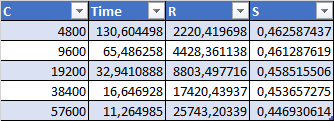
\includegraphics[width=\textwidth]{tabelaBaudrate.png}
\captionof{figure}{Tabela com diferentes valores de Baudrate}

\bigskip
\bigskip

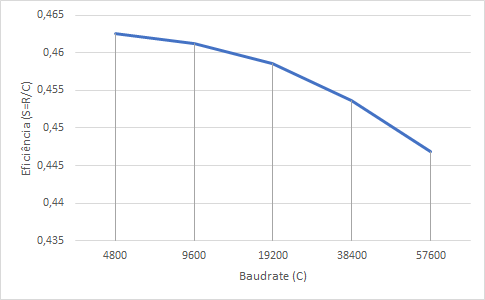
\includegraphics[width=\textwidth]{baudrate.png}
\captionof{figure}{Eficiência em função do Baudrate}

\pagebreak

\subsection{ Anexo XV - Variação do tamanho das tramas}

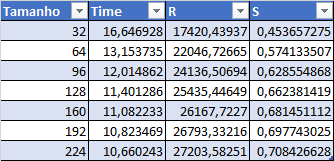
\includegraphics[width=\textwidth]{tabelaTamanho.png}
\captionof{figure}{Tabela com diferentes tamanhos da trama de envio}

\bigskip
\bigskip

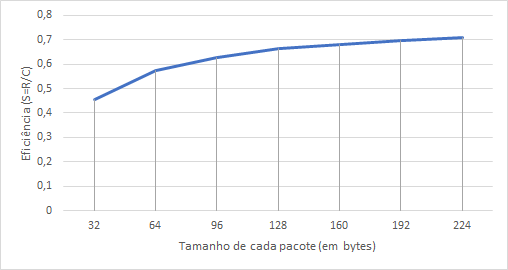
\includegraphics[width=\textwidth]{tamanho.png}
\captionof{figure}{Eficiência em função do tamanho da trama de envio}

\pagebreak

\subsection{ Anexo XVI - Introdução de atraso de propagação}

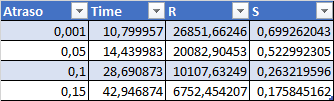
\includegraphics[width=\textwidth]{tabelaAtraso.png}
\captionof{figure}{Tabela com diferentes valores de atraso no envio de tramas}

\bigskip
\bigskip

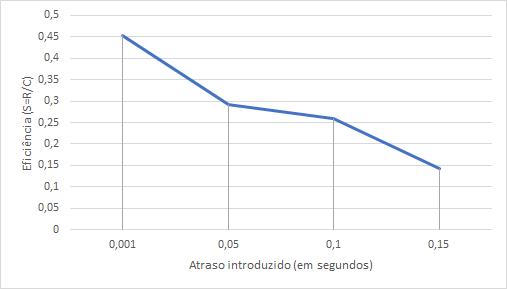
\includegraphics[width=\textwidth]{atraso.png}
\captionof{figure}{Eficiência em função do atraso introduzido}

\pagebreak

\subsection{ Anexo XVII - Introdução de erros nas tramas}

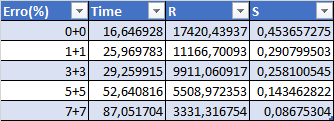
\includegraphics[width=\textwidth]{tabelaErro.png}
\captionof{figure}{Tabela com diferentes valores percentuais de erro introduzido}

\bigskip
\bigskip

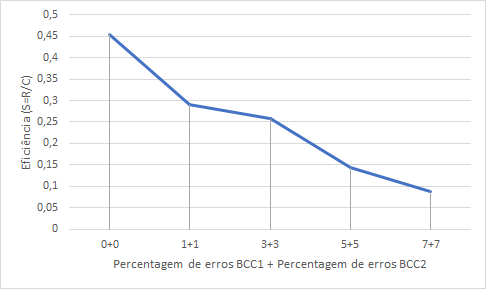
\includegraphics[width=\textwidth]{erro.png}
\captionof{figure}{Eficiência em função da percentagem de erros introduzidos no BCC e BCC2}


	

\end{document}